% Template for ICASSP-2010 paper; to be used with:
%          mlspconf.sty  - ICASSP/ICIP LaTeX style file adapted for MLSP, and
%          IEEEbib.bst - IEEE bibliography style file.
% --------------------------------------------------------------------------
\documentclass{article}
\usepackage{amsmath,graphicx,02460}



\toappear{02460 Advanced Machine Learning, DTU Compute, Autumn 2019}


% Example definitions.
% --------------------
\def\x{{\mathbf x}}
\def\L{{\cal L}}

% Title.
% ------
\title{SegNet on Drone Images: Image Segmentation for Smart Agriculture}
%
% Single address.
% ---------------
\name{			Anders Henriksen, Asger Schultz, Oskar Wiese, 	Mads Andersen,
	Søren Winkel Holm }
\address{s183904, s183912, s183917, s173934, s183911}
%
% For example:
% ------------
%\address{School\\
%	Department\\
%	Address}
%
% Two addresses (uncomment and modify for two-address case).
% ----------------------------------------------------------
%\twoauthors
%  {A. Author-one, B. Author-two\sthanks{Thanks to XYZ agency for funding.}}
%	{School A-B\\
%	Department A-B\\
%	Address A-B}
%  {C. Author-three, D. Author-four\sthanks{The fourth author performed the work
%	while at ...}}
%	{School C-D\\
%	Department C-D\\
%	Address C-D}
%
\begin{document}
%\ninept
%

\maketitle
%
\begin{abstract}
The abstract should appear at the top of the left-hand column of text, about
0.5 inch (12 mm) below the title area and no more than 3.125 inches (80 mm) in
length.  Leave a 0.5 inch (12 mm) space between the end of the abstract and the
beginning of the main text.  The abstract should contain about 100 to 150
words, and should be identical to the abstract text submitted electronically
along with the paper cover sheet.  All manuscripts must be in English, printed
in black ink.
\end{abstract}
%
\begin{keywords}
One, two, three, four, five
\end{keywords}
%
\section{Introduction}
\label{sec:intro}

\subsection{Brief overview of data}
Our data consist of one large, high resolution orthomosaic photo of a sugar cane field formatted as a RGB image. The field has been manually labelled by expert biologist to create a human-ground truth, these labels are represented as a GT-matrix with 3 possible classes. Each pixel is either classified as a crop row (green), weed (yellow), background (red). The large photo is cropped into smaller images and afterwards augmentation techniques are used to gain more data. We will return to the augmentation part later. The images with exclusively black pixels are removed from our data set, and images with some black pixels are ignored when calculating the loss function 
\section{METHODS}
\label{sec:format}


Netværket blev initialiseret

The encoder part of the network creates a rich feature map representing the image content. The more 
layers of max-pooling there are the more translation invariance for robust 
classification can be achieved. The boundary detail is very important when 
dealing with image segmentation. Hence, capturing boundary information in 
the feature maps of the encoder before upsampling is important. This can 
simply be done by storing the whole feature map, but due to memory 
constrains only the maxpooling indices are saved, which is a good 
approximation of the feature maps. 
\subsection{Loss function: Quality over quantity}
Multi-class cross entropy because:
\begin{itemize}
	\item Softmax Network: Minus log likelihood
	\item Can be seen as a classic multiclass classifier -- just on a pixel-by-pixel basis.
\end{itemize}
Weighted cross entropy because:
\begin{itemize}
	\item Unbalanced class distribution: Network has to learn to focus on important pixels: Don't classify everything as dirt.
	\item Initial tests made the network behave as the baseline: Simple features in early layers got were not penalized enough and learning was not stable.
	\item Resampling expensive
\end{itemize}
\subsection{Metrics}
Had to use different metrics because
\begin{itemize}
	\item Not agreement in Image Segmentation papers.
	\item Want to get accuracy on a global scale and on a class scale.
	\item Different metrics important in different fields.
\end{itemize}
The metrics \footnote{https://hal.inria.fr/hal-01581525/document}\footnote{
	http://www.bmva.org/bmvc/2013/Papers/paper0032/paper0032.pdf} 
\begin{itemize}
	\item Global accuracy: Trivial and  not very important because of class imbalance but is good for smoothness
	\item Mean class-wise accuracy: Takes class imbalance into account. Is what is being optimized for in the model.
	\item Mean Intersect over Union: "Jaccard Index".  Found to be better correlated with human classification though still only \(\approx 0.5\). Favours region smoothness highly and not boundary accuracy.
	\item Harmonic mean of precision and recall. To compare to others with same project. Penalizes false positives and gives less credit to true negatives thus being better for unbalanced classes.
\end{itemize}

\subsection{Regularization and Hyperparameters}
Regularization
\begin{itemize}
	\item NN's are prone to overfitting, because they are so flexible
	\item Prevent overfitting $ \to $ better results on test data
	\item Three methods
	\item Dropout: Randomly remove nodes to increase variability. $ p=10 \%$
	\item Data augmentation: Increase size of dataset
	\begin{itemize}
		\item Crop each $ 512\times 512 $ to random $ 256\times 256 $
		\item 50\% chance of flip T/D and 50\% chance of flip L/R
	\end{itemize}
	\item Batch normalization normalizes activations
	\begin{itemize}
		\item Faster convergence
		\item Prevents ReLU from not learning
		\item Introduces noise
		\item Reduces vanishing/exploding gradient problem, as values stay close to 0
	\end{itemize}
\end{itemize}
Hyperparameters
\begin{itemize}
	\item Adaptive learning rate from ADAM optimizer, initialized at $ 2\cdot10^{-4} $
	\item Total: 26 conv + batchnorm + ReLU with dropout, 5 pool/upsample, 1 softmax
	\item 14.7 M parameters in encoder -- significantly lower than 134 M in VGG16 because of no fully-connected layers
	\item Kernel size: $ 3\times 3 $, stride 1, maxpool: $ 2\times 2 $, stride 2
	\item Corresponding padding of 1 to prevent reduction of image size
\end{itemize}



\subsection{Unification of cropped image predictions}
In a real-world application of the field classification a farmer would want a complete and precise segmentation of his whole field at once, such that fertilizer and pesticides can be distributed accordingly. To accomplish this, a reconstruction of the smaller image inferences is neccesary. The most straight forward method of combining the smaller images, by simply lining them up next to each other result is a very rough transition between the smaller inferences. This can be seen in the left side of \ref{fig:earlylatereconstruction}. The blocky nature of the field prediction is caused by a convulutional networks lack of information from neighbouring pixel when inference is performed near the borders of an image. Our way of handling the problem was to increase the cropping size and add overlap when performing the inference. At the cost of computational efficiency more information is available near the borders and a smooth field prediction can be archieved. This can be seen in the right side of \ref{fig:earlylatereconstruction}. A visualization of the reconstruction technique can be seen in appendix \ref{reconstruction_technique}.

\begin{figure}
	\centering
	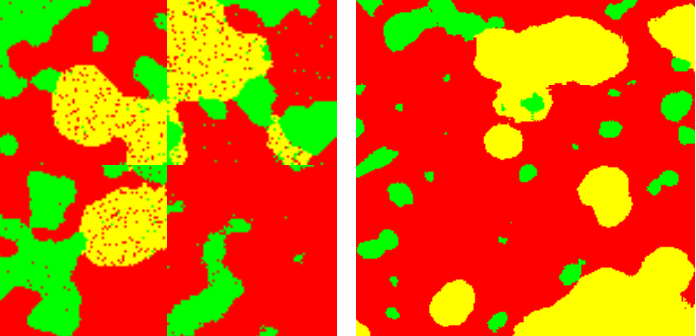
\includegraphics[width=0.9\linewidth]{early_late_reconstruction}
	\caption{\textbf{Left:} Smaller inferences put next to eachother without use of reconstruction techniques. \textbf{Right:} Reconstruction with padding and overlap between smaller inferences.}
	\label{fig:earlylatereconstruction}
\end{figure}

   of doing this  However, it turns out that the prediction quality is of less quality near the boarders of the image. Therefore, a naïve stitching of the cropped images leads to a full-blown image prediction with obvious flaws near the boarders between the cropped images. To solve this problem, we have chosen to increase the size of the cropped images, and infer on these enlarged pictured. In the procedure of joining the enlarged cropped pictures the pictures are cropped again, to avoid the near border areas. This is computationally inefficient, but it works, and since the inference time is not that big, it is an alright solution. For industrial purposes, another approach might be beneficial.




\section{RESULTS}
\label{sec:illust}

% Below is an example of how to insert images. Delete the ``\vspace'' line,
% uncomment the preceding line ``\centerline...'' and replace ``imageX.ps''
% with a suitable PostScript file name.
% -------------------------------------------------------------------------
%\begin{figure}[htb]

%\begin{minipage}[b]{1.0\linewidth}
  %\centering
%  \centerline{\includegraphics[width=8.5cm]{image1}}
%  \vspace{2.0cm}
 % \centerline{(a) Result 1}\medskip
%\end{minipage}
%
%\begin{minipage}[b]{.48\linewidth}
  %\centering
%  \centerline{\includegraphics[width=4.0cm]{image3}}
%  \vspace{1.5cm}
 % \centerline{(b) Results 3}\medskip
%\end{minipage}
%\hfill
%\begin{minipage}[b]{0.48\linewidth}
  %\centering
 % \centerline{\includegraphics[width=4.0cm]{image4}}
%  \vspace{1.5cm}
 % \centerline{(c) Result 4}\medskip
%\end{minipage}
%
%\caption{Example of placing a figure with experimental results.}
%\label{fig:res}
%
%\end{figure}

% To start a new column (but not a new page) and help balance the last-page
% column length use \vfill\pagebreak.
% -------------------------------------------------------------------------
%\vfill
%\pagebreak


\section{DISCUSSION}
\label{sec:foot}
\subsection{Comparison of different image segmentation neural networks}
\begin{itemize}
	\item Several competing network structures with high performance in image segmentation. U-net, FCN, DeepLabv1, DeconvNet
	\item Purpose of SegNet, efficient
	\item 3 out of the 4 mentioned uses the encoder from the famous VGG16 paper, but differ in decoder.
	\item FCN, No decoder -> Blocky segmentation, but very efficient in inference time.
	\item DeconvNet, Deconvolution and fully connected layers. 
	\item U-Net, (different purpose), skip connections. 
	\item Main takeaway  
	\item (Deeplabv-LargeFOV \& FCN)
	
\end{itemize}
\cite{seg}

\subsection{Extension of network}


\subsection{Conclusion}

\bibliographystyle{IEEEbib}
\bibliography{refs}

\subsection{Appendix}
\begin{figure}
	\centering
	\includegraphics[width=0.7\linewidth]{"reconstruction DL"}
	\caption{Reconstruction of the smaller inferences into a unified field prediction.}
	\label{reconstruction_technique}
\end{figure}



\end{document}
